%%% Template originaly created by Karol Kozioł (mail@karol-koziol.net) and modified for ShareLaTeX use

\documentclass[a4paper,11pt]{article}

\usepackage[T1]{fontenc}
\usepackage[utf8]{inputenc}
\usepackage{graphicx}
\usepackage{xcolor}

\renewcommand\familydefault{\sfdefault}
\usepackage{tgheros}
\usepackage[defaultmono]{droidmono}

\usepackage{url}
\usepackage{enumerate}

\usepackage{amsmath,amssymb,amsthm,textcomp}
\usepackage{enumerate}
\usepackage{multicol}
\usepackage{tikz}

\usepackage{geometry}
\geometry{left=25mm,right=25mm,%
bindingoffset=0mm, top=20mm,bottom=20mm}


\linespread{1.3}

\newcommand{\linia}{\rule{\linewidth}{0.5pt}}

% custom theorems if needed
\newtheoremstyle{mytheor}
    {1ex}{1ex}{\normalfont}{0pt}{\scshape}{.}{1ex}
    {{\thmname{#1 }}{\thmnumber{#2}}{\thmnote{ (#3)}}}

\theoremstyle{mytheor}
\newtheorem{defi}{Definition}

% my own titles
\makeatletter
\renewcommand{\maketitle}{
\begin{center}
\vspace{2ex}
{\huge \textsc{\@title}}
\vspace{1ex}
\\
\linia\\
\@author \hfill \@date
\vspace{4ex}
\end{center}
}
\makeatother
%%%

% custom footers and headers
\usepackage{fancyhdr}
\pagestyle{fancy}
\lhead{}
\chead{}
\rhead{}
\lfoot{Projectlet hanoi}
\cfoot{}
\rfoot{Page \thepage}
\renewcommand{\headrulewidth}{0pt}
\renewcommand{\footrulewidth}{0pt}
%

% code listing settings
\usepackage{listings}
\lstset{
    language=Python,
    basicstyle=\ttfamily\small,
    aboveskip={1.0\baselineskip},
    belowskip={1.0\baselineskip},
    columns=fixed,
    extendedchars=true,
    breaklines=true,
    tabsize=4,
    prebreak=\raisebox{0ex}[0ex][0ex]{\ensuremath{\hookleftarrow}},
    frame=lines,
    showtabs=false,
    showspaces=false,
    showstringspaces=false,
    keywordstyle=\color[rgb]{0.627,0.126,0.941},
    commentstyle=\color[rgb]{0.133,0.545,0.133},
    stringstyle=\color[rgb]{01,0,0},
    numbers=left,
    numberstyle=\small,
    stepnumber=1,
    numbersep=10pt,
    captionpos=t,
    escapeinside={\%*}{*)}
}

%%%----------%%%----------%%%----------%%%----------%%%

\begin{document}

\title{Towers of Hanoi}

\author{rs@toprllc.com}

\date{\today}

\maketitle

\section*{Introduction}

It is not surprising that as the size of a problem - however \textbf{the size} is defined, will determine the cost of a solution. For a given problem, there may be multiple solutions possible and we may have to understand the cost before settling on the solution. Facial recognition for example is such a problem where there may be a large database to search for a match. Confronted by a choice, algorithms need to be evaluated before one is chosen for implementation.


\paragraph{}In this projectlet, the familiar problem \textbf{Towers of Hanoi} is used to explore such ideas. \url{https://en.wikipedia.org/wiki/Tower_of_Hanoi} defines the basic problem and outlines a \textbf{recursive} and an \textbf{iterative} solution. This can be implemented with appropriate instrumentation to compare the performance.

\paragraph{}\textbf{Wikipedia} article referenced above also points to several extensions e.g. higher number of pegs and other rule set governing the moves.

\paragraph{}The goal is to experiment with ideas for instrumentation for performance comparisons. In particular, it is posited that algorithm visualization graphically gives a good insight into the performance of algorithms - in comparison with a simpler text output based comparisons. As we explore visualizations, the separation of the algorithm from the visualization becomes a topic to explore as well. A clean separation will enable substitution of visualization techniques and toolkits without compromising the algorithm.

\section*{Initial approach}

The two factors that are impacted by the size of the problem are execution time and memory usage. A reasonable assumption might be that both recursive and iterative solutions utilize the same data structure (which may not always be true). Analytically it has been proven that the minimal number of moves for n disks is $2^{(n)} - 1$. Implementation of both the recursive and the iterative algorithms, illustrating the instrumentation techniques demonstrates this.

\paragraph{}
 In the case of a recursive approach, the depth of recursion will be a proxy for space since each invocation requires stack growth.
 
\subsection*{Results}

\paragraph{}
For a recursive solution, we find that the maximum depth is the same as the number of disks. The total number of moves however is $2^{(n)} - 1$.

\fbox{%
    \parbox{30em}{%
    Total no of moves 65535 Iterations 0 Max Depth 16
    }%
}

\paragraph{}
For an iterative solution, the number of disk moves is still the same ie $2^{(n)} - 1$.

\fbox{%
    \parbox{30em}{%
    Total no of moves 65535 Iterations 21845 Max Depth 0
    }%
}
More experimentation leads to the following:
\begin{table}[h!]
\begin{center}
\begin{tabular}{ | c | c | }
\hline
 Disks & Iterations \\
 \hline
 16 & 21845 \\ 
 20 & 349525 \\  
 24 & 5592405 \\
 28 & 89478485 \\
 \hline
\end{tabular}
\caption{Number of disks vs Number of iterations required to solve}
\label{table:1}
\end{center}

\end{table}

\section*{Algorithm Visualization}

The impact of the performance implications would be readily apparent if the execution is visualized. For example, if the moves of the disks are presented graphically, and every move is presented in a graphical interface, the sheer number of moves and the time it takes would be clear. By varying the number of disks, we can immediately appreciate the relation. The ability 
to pause/resume the progress proves to be highly educational

\subsection*{Animation - fyne graphical library}
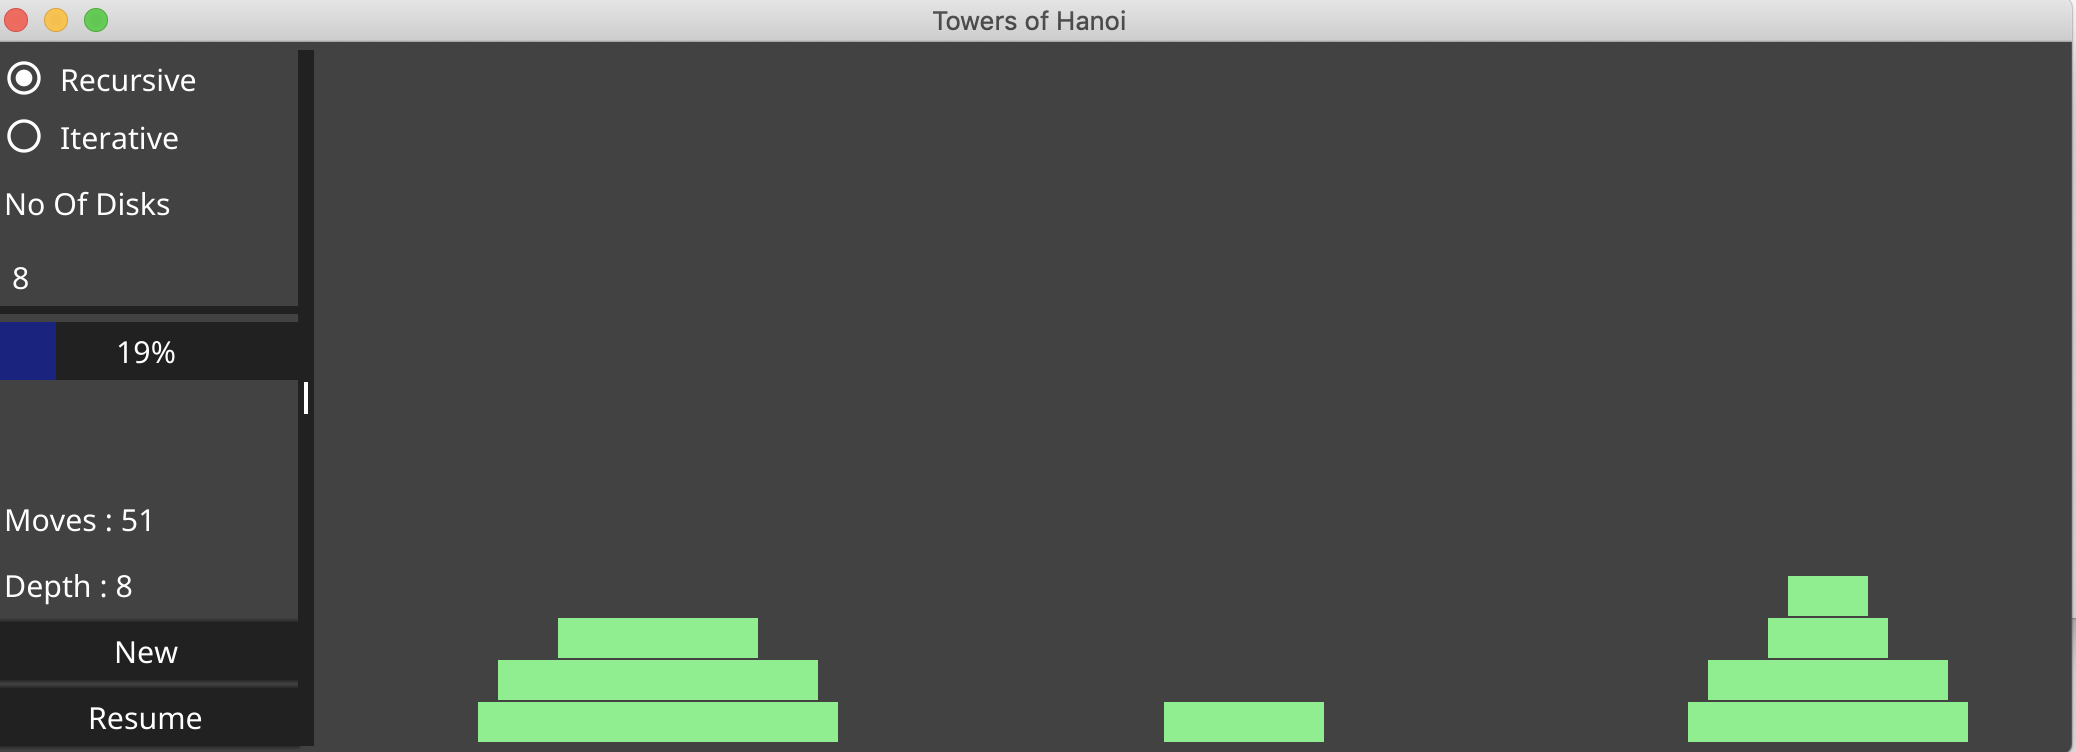
\includegraphics[width=6in]{TowersOfHanoi.png}

\subsection*{Animation - gtk3 library}
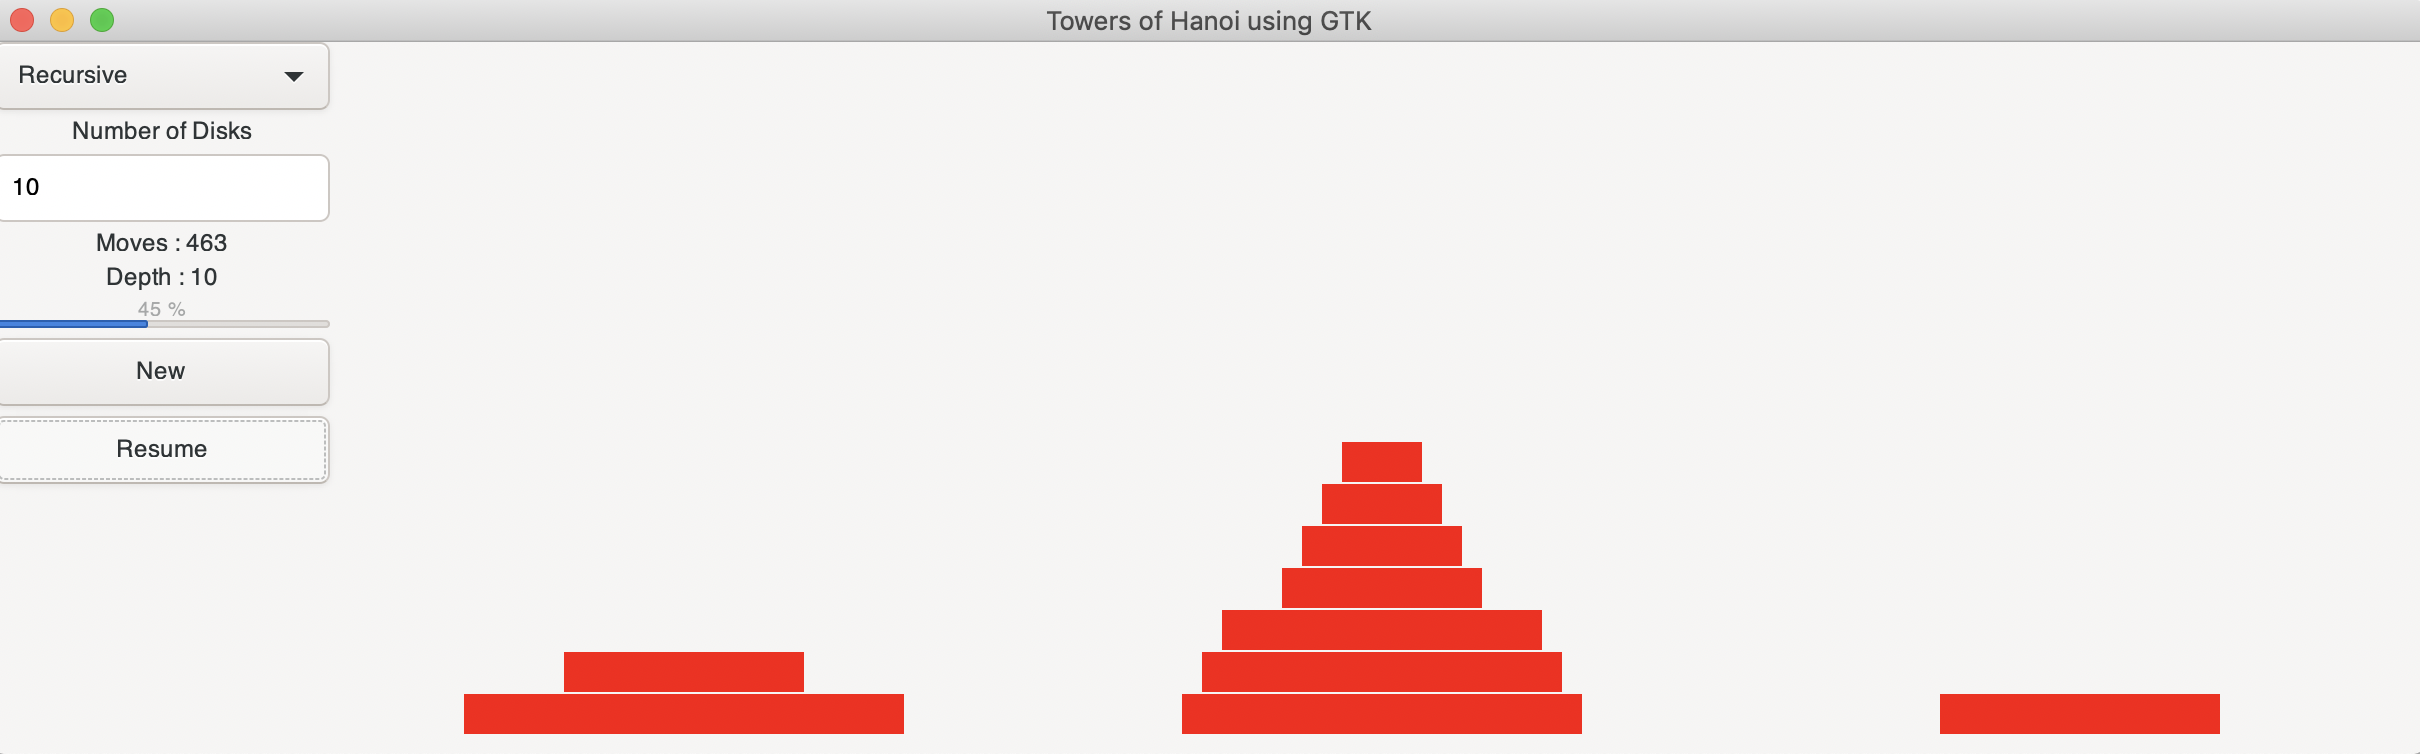
\includegraphics[width=6in]{gtkexample.png}

\section*{Implementation}

\subsection*{Example Project}

An example project has been developed to illustrate the concepts - with the following specifications:
\paragraph{}
\fbox{%
    \parbox{40em}{%

usage: hanoi <number of disks> [iterative] [graphic]

              iterative - use the iterative solution.
              graphic - present the solution graphically
 

     }%
}

\paragraph{}

An implementation in \textbf{go} language using \textbf{fyne} (\url{https://fyne.io/}) library for gui has been developed and is available for exploration and enhancements. The project also incorporates an alternative implementation using the \textbf{gtk3} framework (\url{https://github.com/gotk3/gotk3}).

\fbox{%
    \parbox{45em}{%
    \url{https://sourceforge.net/p/gohanoi/code/ci/master/tree/}
    }%
}

\end{document}
